\newpage
\section{Diffusion coefficient}

Using the data from table \ref{tab:tabla2}, the diffusion coefficient was calculated with the Arrhenius relation:
\begin{align}
    \label{eq:1}
    D&=D_0 exp\left(-\dfrac{\Delta H}{RT}\right),
\end{align}
where $D$ is the Diffusion coefficient, $D_0$ is a pre-exponential factor, $\Delta H$ is the activation entalphy of diffusion in $k J/mol$ (which is also represented as $Q$), R is the ideal gas constant ($8,314 J/K\cdot mol$) and T is the temperature in Kelvin \citep{diff}. \\

The linearization of Arrhenius relation can be made by taking the logarithm on both sides of equation \eqref{eq:1}, which yields:
\begin{align}
  \label{eq:2}
  ln(D)&=-\dfrac{\Delta H}{R}\dfrac{1}{T} + ln(D_0),
\end{align}
which is a linear equation where the slope is given by $-\Delta H/R$ and the intercept in the y-axis is given by $ln(D_0)$. \\

Considering that all systems have different temperature ranges (\ref{tab:tabla2}), to proceed with the calculations, a new temperature range was chosen, from $450$ to $1950$ K, so that all systems use the same temperature range and can be compared with each other. The new temperature range was used to calculate $D$ for all systems, with a sample of 100 points evenly spaced, and the parameters of $D_0$, $Q$ and $R$ using equation \eqref{eq:1}.\\

The results for the diffusion coefficient for all systems are presented in figure \ref{fig:diffusion}. Figure \ref{fig:d} shows the diffusion coefficient for all systems as a function of temperature, from $450$ to $1950$K; the linearization of Arrhenius relation is shown in figure \ref{fig:lnd}, where the logarithm of the diffusion coefficient is plotted as a function of the inverse of the temperature.

\begin{figure}[h]
 \centering
 \captionsetup{justification=centering,margin=2cm}
  \subfloat[]{
   \label{fig:d}
    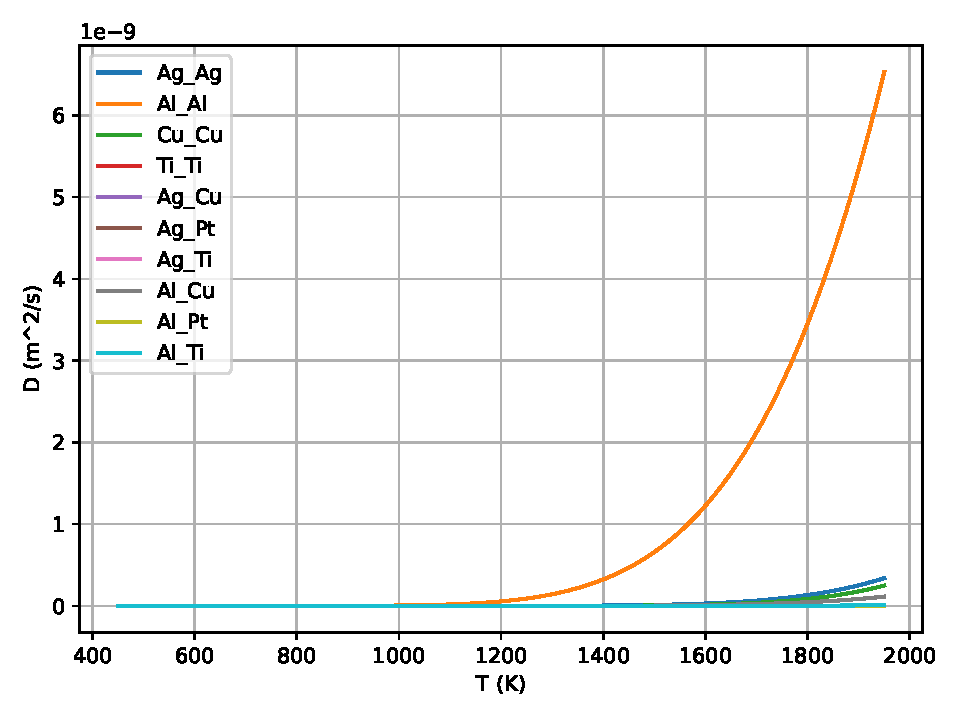
\includegraphics[width=0.5\textwidth]{graficas/D(T).pdf}}
  \subfloat[]{
   \label{fig:lnd}
    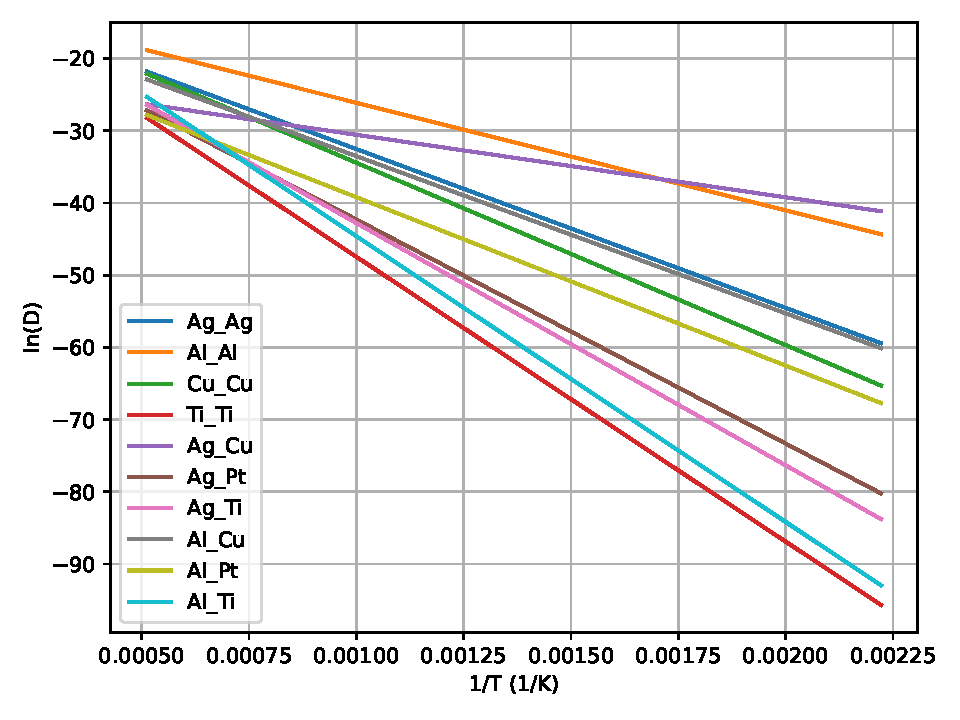
\includegraphics[width=0.5\textwidth]{graficas/ln(D).pdf}}
 \caption{a) Diffusion coefficient $D$ ($m^2/s)$ as a function of temperature $T$ (K) and b) logarithm of the diffusion coefficient $ln(D)$ as a function of the inverse of temperature $1/T$ ($K^{-1}$). \\
 \textit{Source: Data from \citep{kakusan}, visualization by the author (code available at \citep{mygit}).}}
 \label{fig:diffusion}
\end{figure}


\newpage
\subsection{Self diffusion}

The self-diffusing systems are Ag-Ag, Al-Al, Cu-Cu and Ti-Ti. The plot for the logarithm of the diffusion coefficient as a function of the inverse of the temperature are shown in figure \ref{fig:selfdiff_lnd}.  
\begin{figure}[h]
 \centering
 \captionsetup{justification=centering,margin=2cm}
  \subfloat[]{
   \label{fig:}
    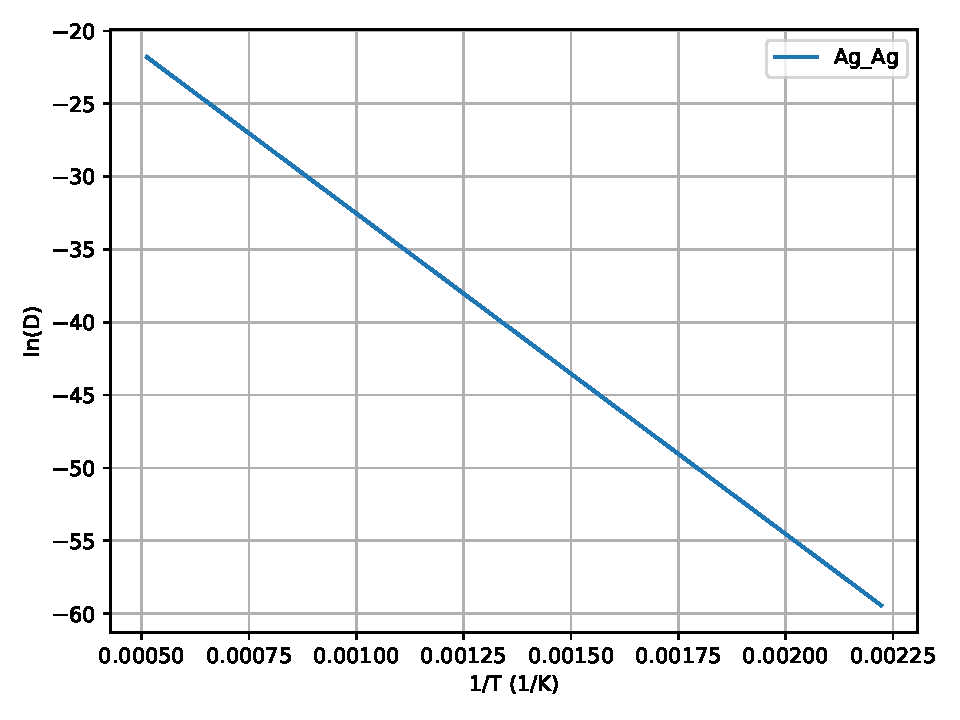
\includegraphics[width=0.5\textwidth]{graficas/Ag_Ag_ln(D).pdf}}
  \subfloat[]{
   \label{fig:sigma4}
    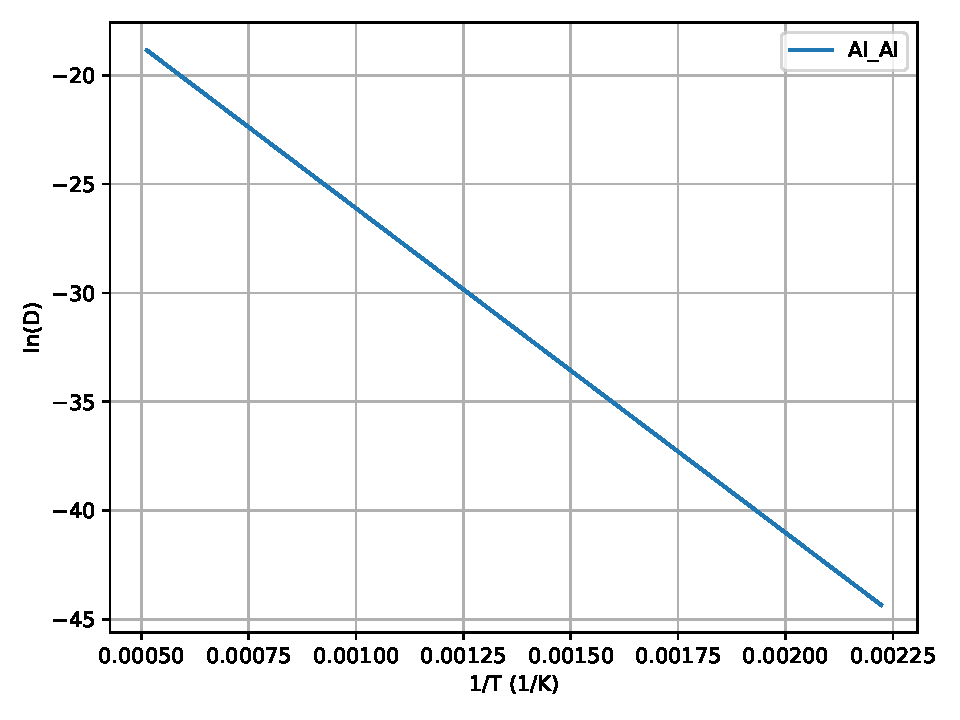
\includegraphics[width=0.5\textwidth]{graficas/Al_Al_ln(D).pdf}} \\
  \subfloat[]{
   \label{fig:}
    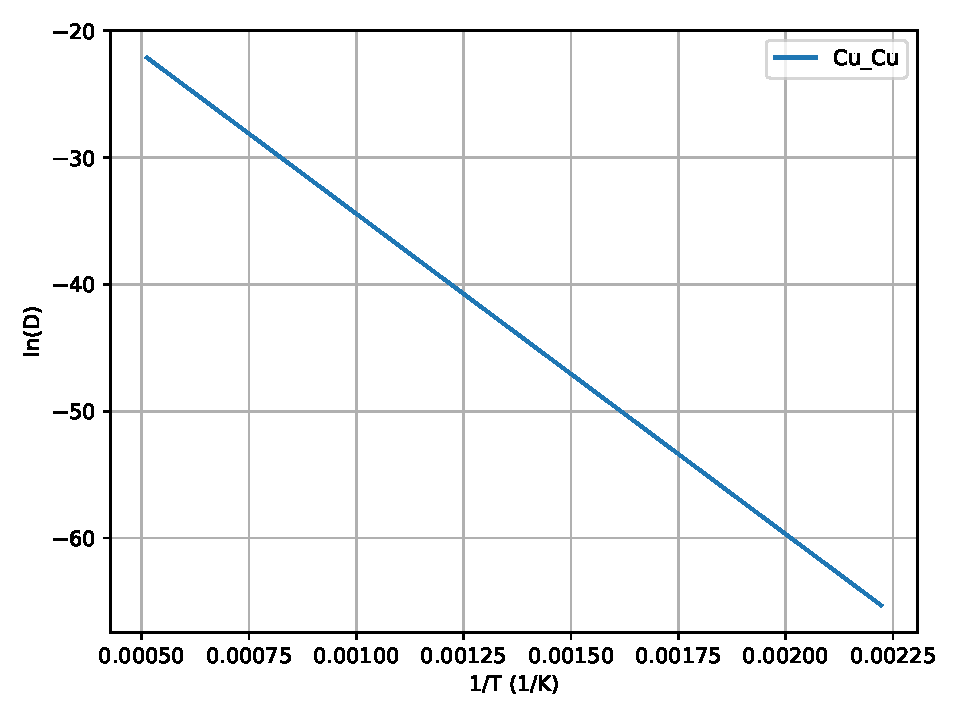
\includegraphics[width=0.5\textwidth]{graficas/Cu_Cu_ln(D).pdf}}
  \subfloat[]{
   \label{fig:sigma4}
    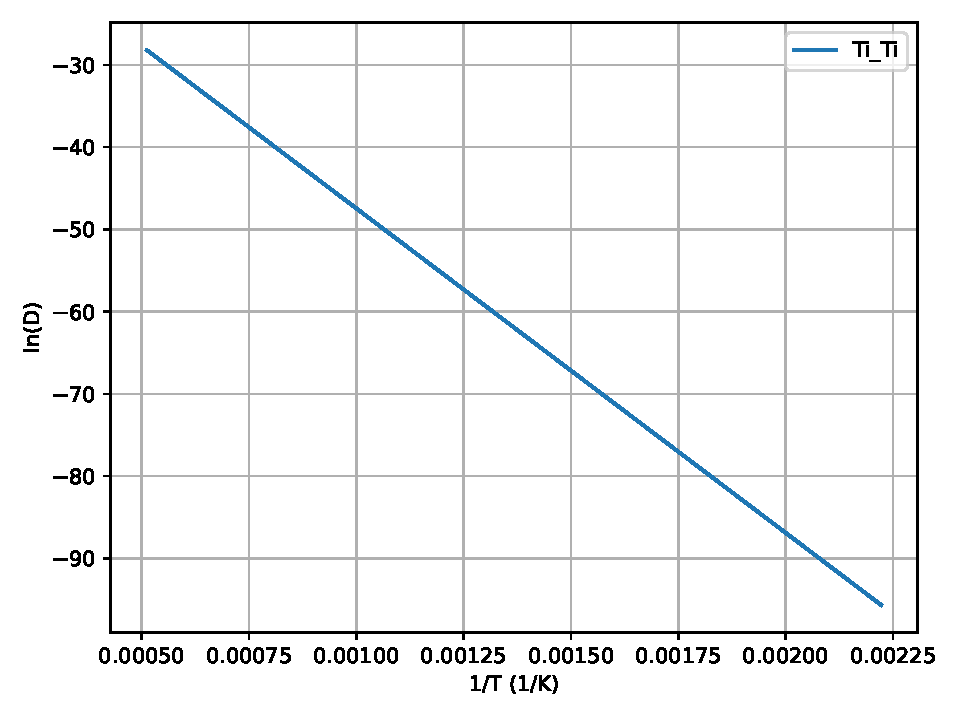
\includegraphics[width=0.5\textwidth]{graficas/Ti_Ti_ln(D).pdf}}
 \caption{Logarithm of the diffusion coefficient for self-diffusing systems: a) silver, b) aluminum, c) copper and d) titanium.\\ 
 \textit{Source: Data from \citep{kakusan}, visualization by the author (code available at \citep{mygit}).}}
 \label{fig:selfdiff_lnd}
\end{figure}

%\newpage
\subsection{Solute diffusion}

\begin{figure}[h]
 \centering
 \captionsetup{justification=centering,margin=2cm}
  \subfloat[]{
   \label{fig:}
    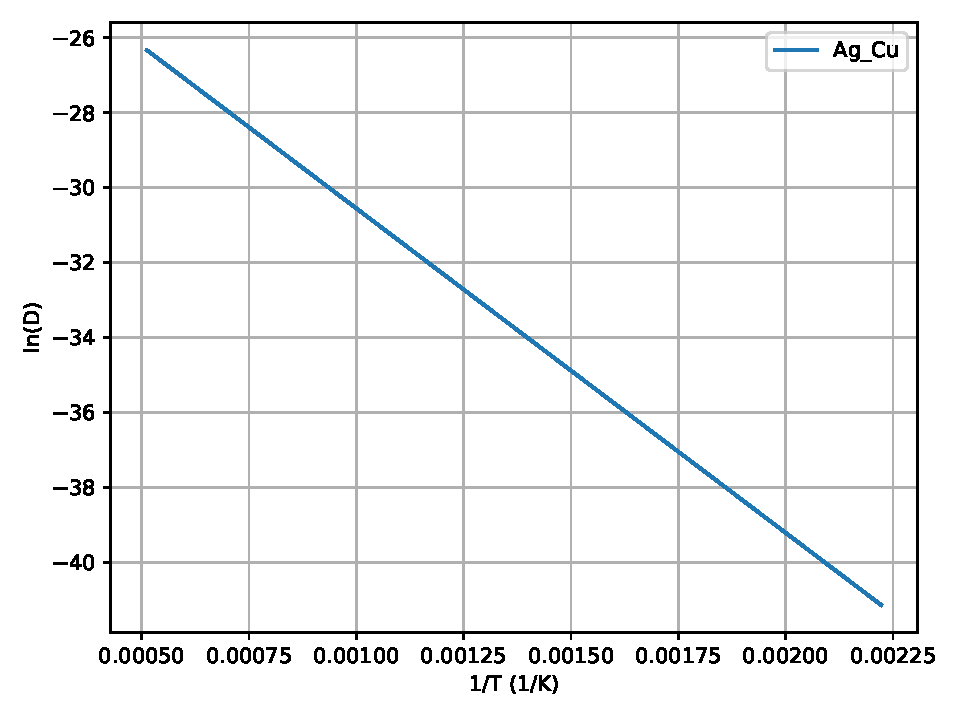
\includegraphics[width=0.5\textwidth]{graficas/Ag_Cu_ln(D).pdf}}
  \subfloat[]{
   \label{fig:sigma4}
    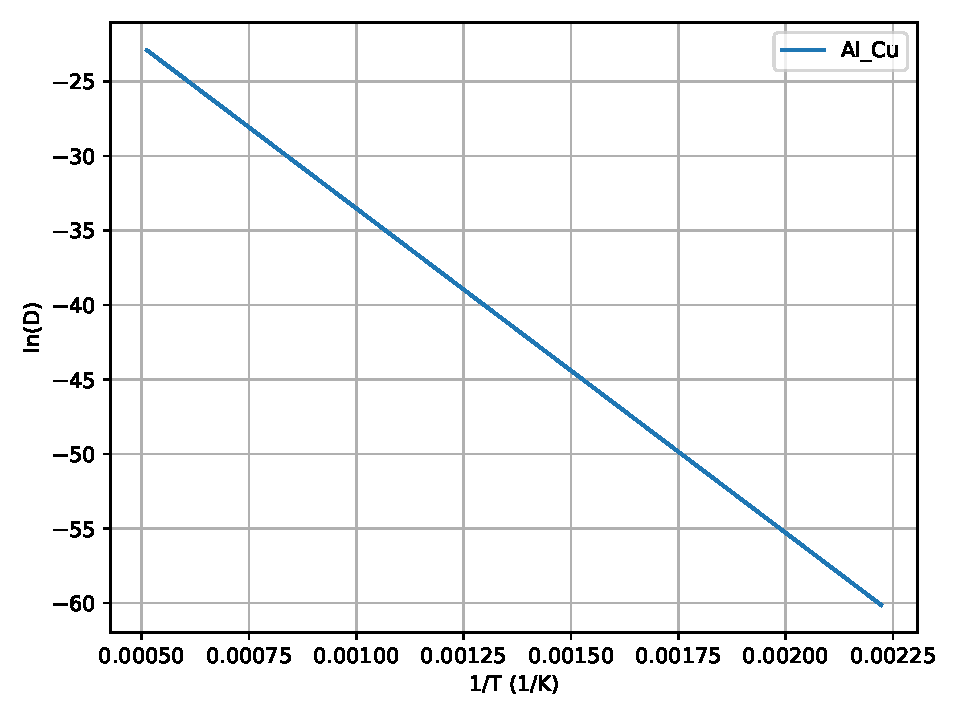
\includegraphics[width=0.5\textwidth]{graficas/Al_Cu_ln(D).pdf}} \\
  \subfloat[]{
   \label{fig:sigma4}
    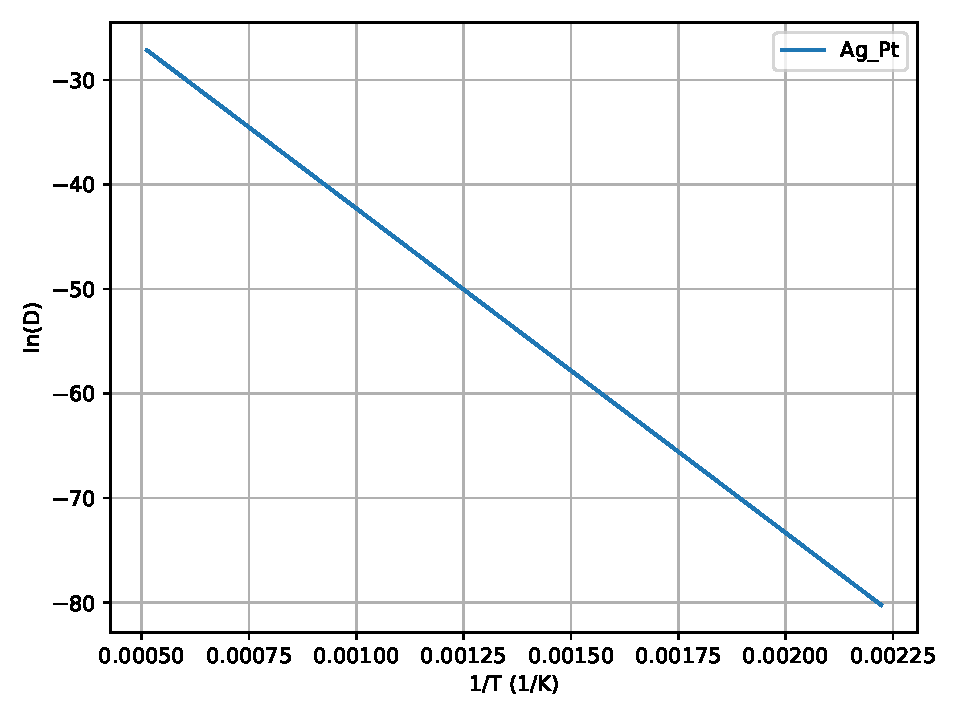
\includegraphics[width=0.5\textwidth]{graficas/Ag_Pt_ln(D).pdf}}
  \subfloat[]{
   \label{fig:sigma4}
    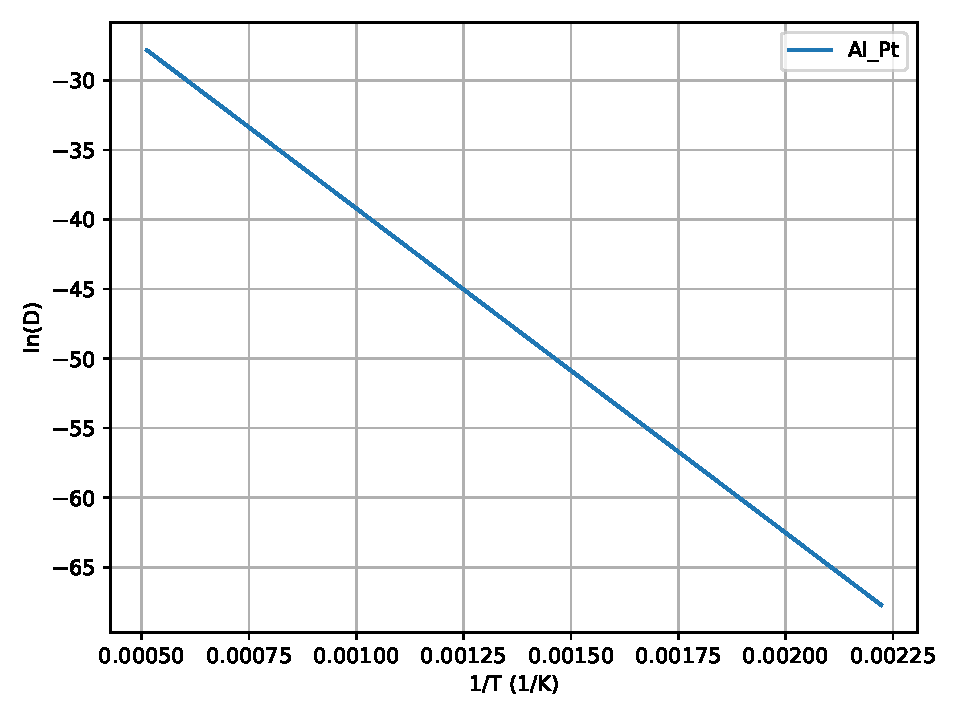
\includegraphics[width=0.5\textwidth]{graficas/Al_Pt_ln(D).pdf}} \\
  \subfloat[]{
   \label{fig:sigma4}
    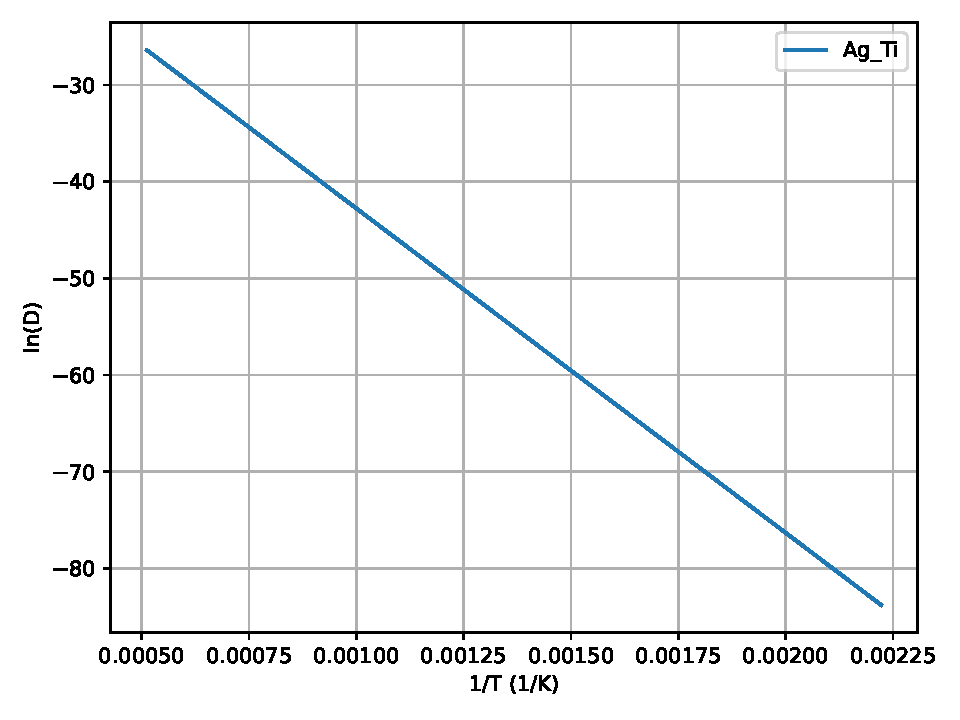
\includegraphics[width=0.5\textwidth]{graficas/Ag_Ti_ln(D).pdf}}
  \subfloat[]{
   \label{fig:sigma4}
    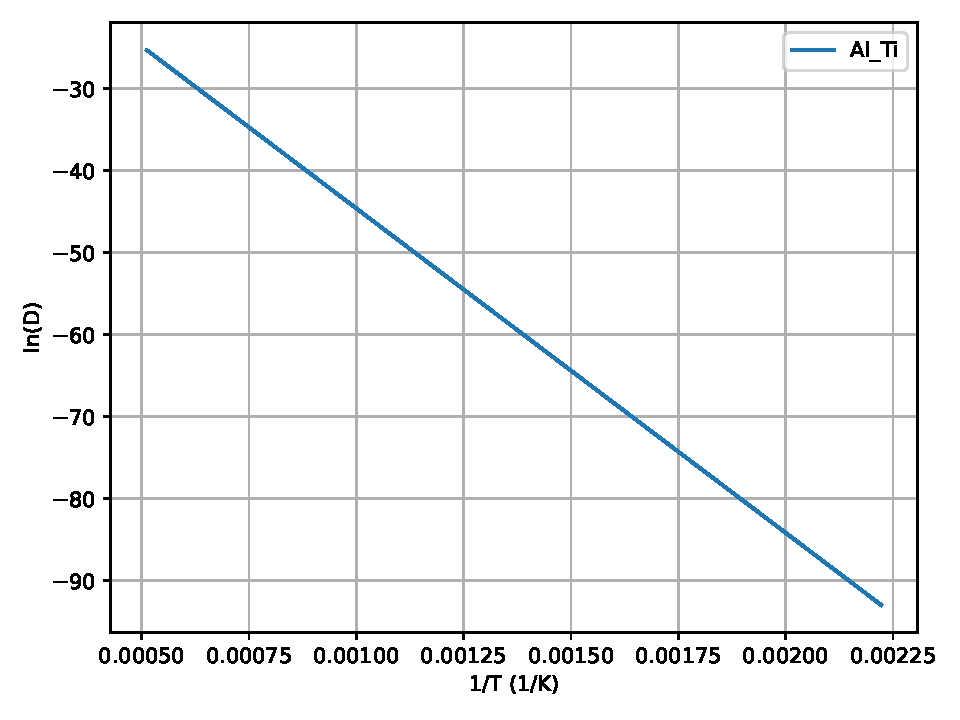
\includegraphics[width=0.5\textwidth]{graficas/Al_Ti_ln(D).pdf}}
 \caption{Logarithm of the diffusion coefficient for the systems: copper diffusing in a) silver and b) aluminum; platinum diffusing in c) silver and d) aluminum; and platinum diffusing in f) silver and g) aluminum.\\ 
 \textit{Source: Data from \citep{kakusan}, visualization by the author (code available at \cite{mygit}).}}
 \label{fig:sigmas}
\end{figure}
